%% ----------------------------------------------------------------
%% InvestigationVision.tex
%% ---------------------------------------------------------------- 
\chapter{Investigation into Vision Algorithms} \label{Chapter:InvestigationVision}

\section{Comparison}
\inote{find some references to back these claims up}
\inote{Talk about how to compare images and TEST them all. Make a final comparison to decide on which will be used}
In computer vision, there are many different ways of comparing two similar images. These include the sum of absolute differences (S.A.D.) (\cite{Hamzah:DistanceDetection}), the sum of squared differences (S.S.D.), normalised cross correlation (N.C.C.) and enhanced normalised cross correlation (E.N.C.C.)

%Explanation of how they work
\subsection{Sum of Absolue Differences}

Given two indentically sized matricies, $A, B$ of dimensions $i,j$, SAD is defined as
\begin{equation}
SAD = \sum\limits_{I=0}^i \sum\limits_{J=0}^j A[I,J] - B[I,J] 
\end{equation}

\subsection{Sum of Squared Differences}
\begin{equation}
SSD = \sum\limits_{I=0}^i \sum\limits_{J=0}^j (A[I,J] - B[I,J] )^2
\end{equation}

\subsection{NCC}
%http://www.bmva.org/bmvc/1998/pdf/p125.pdf
\subsection{ENCC}
%http://xanthippi.ceid.upatras.gr/people/evangelidis/encc/
%test and compare
\subsection{Comparison}



\section{Range Finding}
\inote{Derive the range finding eauations and test the fuck out of it}

\subsection{Derivations}

By using two images sepearted by a horizontal difference, the range of an object can be found given some characteristics of the camera. The following is a derivation of the equations used to calculate distance. 

The problem is broken down into 3
\begin{enumerate}
\item Object is between the cameras (Figure \ref{problem_between})
\item Object is directly infront of a camera
\item Object is in left or right hand sides of both images
\end{enumerate}

\begin{figure}
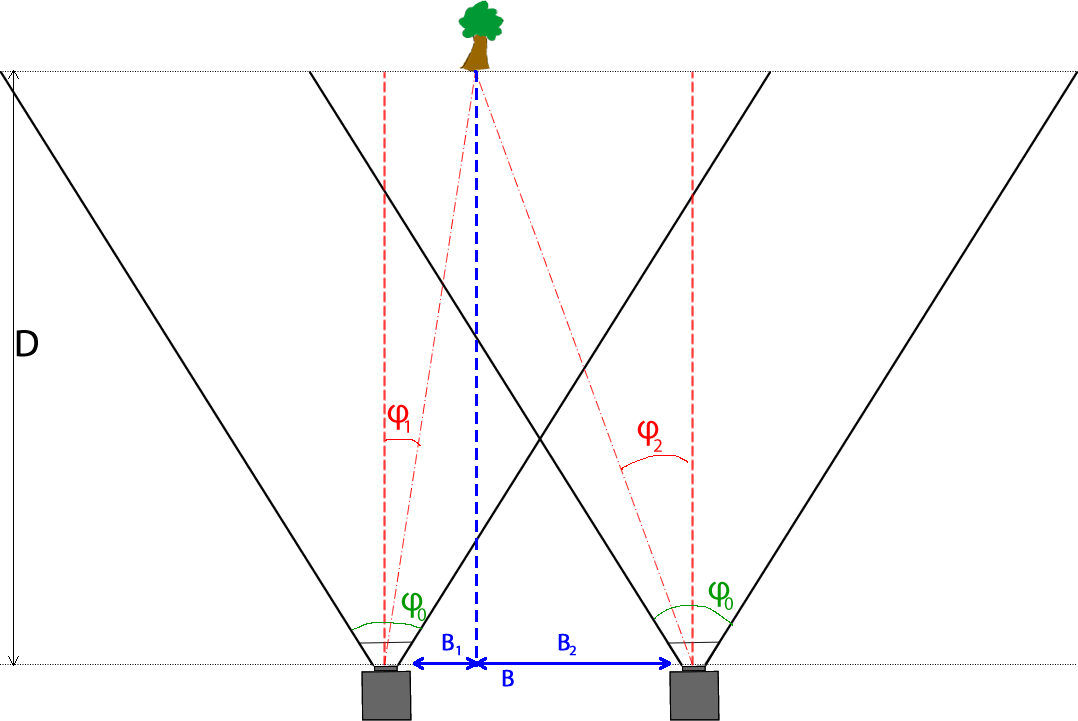
\includegraphics[width=\textwidth,height=\textheight,keepaspectratio]{Figures/problem1.png}
\caption{Problem 1 - Object is between the Cameras}
\label{problem_between}
\end{figure}

\subsubsection{Object is between the Cameras}
Derivation from \cite{Mrovlje:Distance_Stereoscopic}.
\begin{equation} \label{eq:B}
B = B_{1} + B_{2} = D\tan(\varphi_{1}) + D\tan(\varphi_{2})
\end{equation}

\begin{equation} \label{eq:D}
D = \frac{B}{\tan(\varphi_{1}) + \tan(\varphi_{2})}
\end{equation}


\begin{figure}
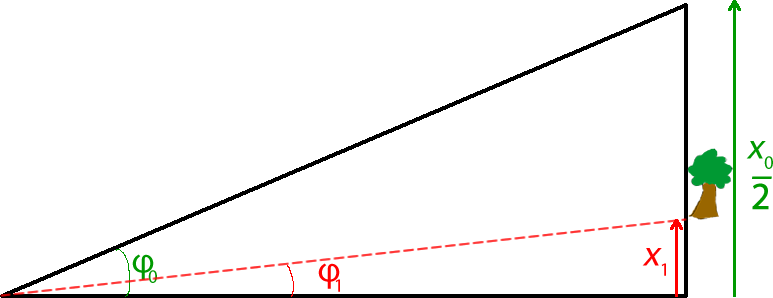
\includegraphics[width=\textwidth,height=\textheight,keepaspectratio]{Figures/left_simplified.png}
\caption{Problem 1 : Left Camera Simplified}
\label{Left_Simplified}
\end{figure}

\begin{equation} \label{eq:phi}
D\tan(\frac{\varphi_{0}}{2}) = x_{0} / 2
\end{equation}

\begin{equation} \label{eq:phi1}
D\tan(\varphi_1) = x_1
\end{equation}

Dividing \eqref{eq:phi1} by \eqref{eq:phi}

\begin{equation} \label{eq:tanovertan}
\frac{\tan(\varphi_1)}{\tan(\frac{\varphi_0}{2})} = \frac{2x_1}{x_0}
\end{equation}

\begin{equation} \label{eq:phionesolved}
\tan(\varphi_1) = \frac{2x_1\tan(\frac{\varphi_0}{2})}{x_0}
\end{equation}

It can also be shown that for the right camera:

\begin{equation} \label{eq:phitwosolved}
\tan(\varphi_2) = \frac{-2x_2\tan(\frac{\varphi_0}{2})}{x_0}
\end{equation}

Substitution equations \eqref{eq:phionesolved} and \eqref{eq:phitwosolved} into \eqref{eq:D} gives

\begin{equation} \label{eq:Distance1}
D = \frac{Bx_0}{2\tan(\frac{\varphi_0}{2})(x_1 - x_2)}
\end{equation}


\subsubsection{Object is infront of a camera}


\subsubsection{Object is to the same side in each camera}

\begin{figure}
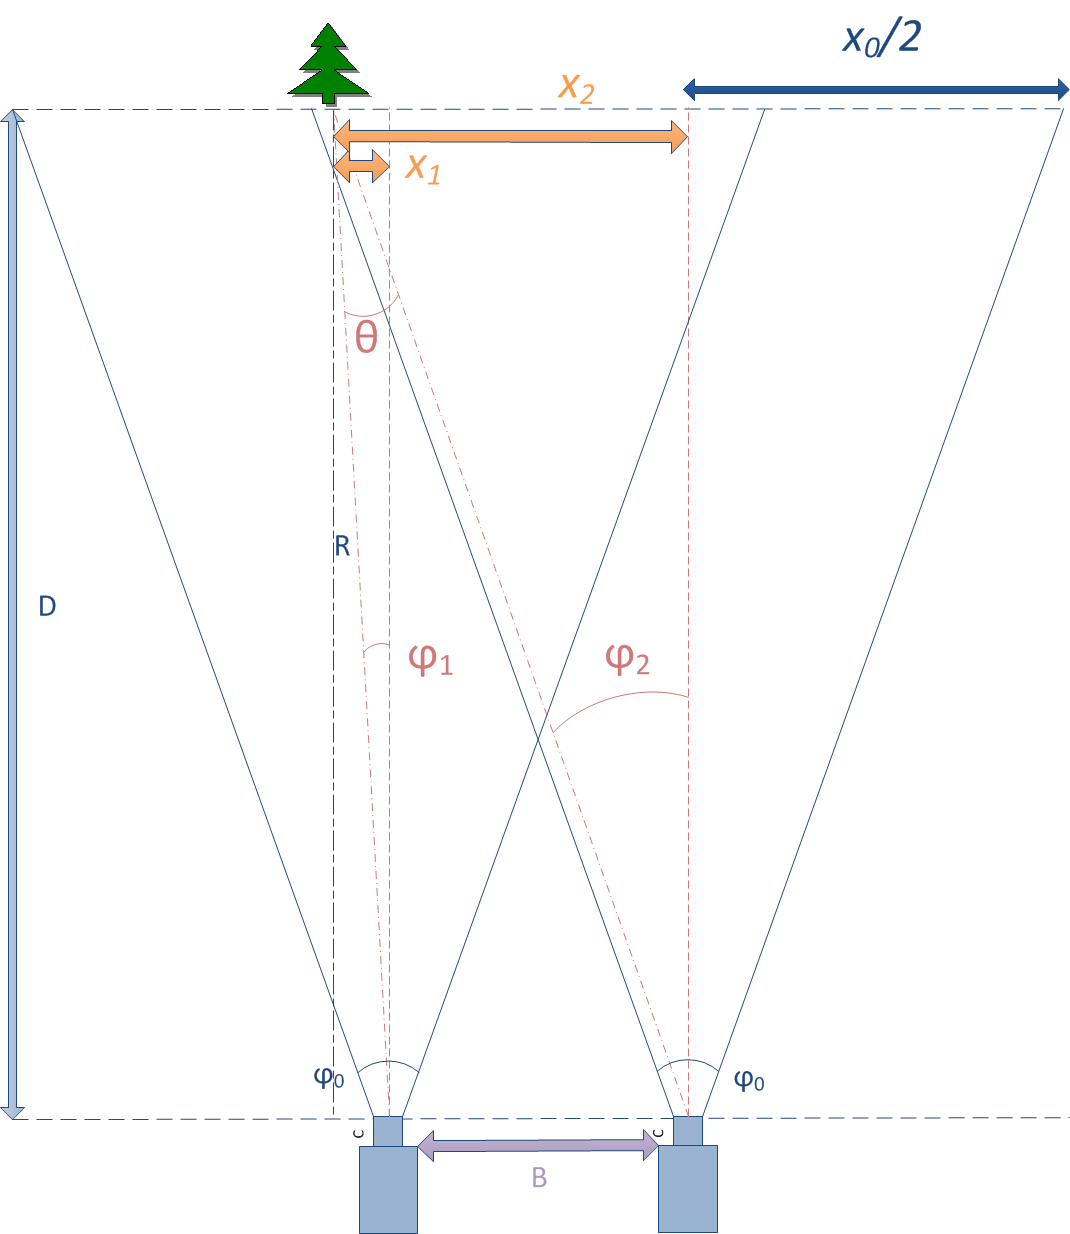
\includegraphics[width=\textwidth,height=\textheight,keepaspectratio]{Figures/problem2.png}
\caption{Problem 3 - Object is to the same side in both cameras}
\label{problem_between}
\end{figure}
